%=============================================================================
%  Part~I: Confound-Controlled Susceptibility and a Three-Stage Validation Ladder
%  IEEE journal format (IEEEtran, two column).
%
%  Build:  tectonic part1.tex
%
%  Generated by scripts/split_journal.py from paper/paper_journal_v2.tex.
%  Every number and figure traces to a script in ../../scripts; none is entered
%  by hand. Edit the source manuscript and re-run the splitter, not this file.
%=============================================================================
\documentclass[journal]{IEEEtran}

\usepackage[T1]{fontenc}
\usepackage{amsmath,amssymb,amsfonts}
\usepackage{graphicx}
\usepackage{booktabs}
\usepackage{multirow}
\usepackage{array}
\usepackage{xcolor}
\usepackage{tikz}
\usetikzlibrary{positioning,arrows.meta,fit,backgrounds}
\usepackage{caption}
\usepackage{subcaption}
\captionsetup[sub]{font=small}
\usepackage[numbers,sort&compress]{natbib}
\usepackage[hidelinks]{hyperref}
\usepackage{siunitx}
\sisetup{detect-all,group-separator={,}}
\usepackage{balance}

\renewcommand{\arraystretch}{1.15}

\newcommand{\Sx}{S(\mathbf{x})}
\newcommand{\Tt}{T(t)}
\newcommand{\Rxt}{R(\mathbf{x},t)}

\begin{document}

\title{Spatiotemporal Flood Risk Modelling Under a Single-Orbit SAR Constraint, Part~I: Confound-Controlled Susceptibility and a Three-Stage Validation Ladder}

% Author identities removed for anonymous review. Restore before camera-ready.
\author{}

\maketitle

\begin{abstract}
Over Dakshina Kannada, Karnataka, exactly one Sentinel-1 orbit
covers the district on a strict twelve-day cycle, so no individual flood there
can be mapped from synthetic aperture radar (SAR): a flash flood rises and
recedes inside the revisit gap. This paper, the first of two, treats that
constraint as the design premise and builds the static half of a two-stage risk
model, $\Rxt=\Sx\cdot\Tt$. A multi-temporal SAR flood-\emph{frequency} inventory
replaces the single-event map that the revisit interval forbids. A
remote-sensing confound is then identified and removed: a model given land cover
and NDVI reaches ROC-AUC 0.9878, but SHAP shows it has learned that closed
canopy hides water from SAR, not flood physics. The terrain-and-rainfall model
scores 0.9625 on a random split, 0.9474 under spatial-block cross-validation,
and 0.871 transferring to a held-out city window never seen in training, where
its highest-susceptibility tenth contains 49.5\% of all SAR-observed flooding.
We show the calibrated score is tied to the balanced training prior and must not
be read as a flood probability without correction. The dynamic trigger $\Tt$,
keyed to India Meteorological Department rainfall categories and fitted to no
event, ranks two documented floods above ordinary and dry conditions but
separates a flood from a heavy-rain non-flood day by only 0.011, a margin
governed almost entirely by its antecedent-saturation term. Each stricter
validation protocol lowers the headline number, and we report the descent rather
than the first figure. Part~II applies the resulting risk surface to emergency
routing and dispatch.
\end{abstract}

\begin{IEEEkeywords}
Flood susceptibility, synthetic aperture radar, Sentinel-1, spatial cross-validation, explainable AI, probability calibration, Google Earth Engine.
\end{IEEEkeywords}

\section{Introduction}
\label{sec:intro}

Flooding is the most frequently recurring natural hazard in India, and the
country's south-western coastal belt concentrates several of the mechanisms that
make it difficult to forecast at a useful spatial scale. Dakshina Kannada
district, centred on the port city of Mangaluru in coastal Karnataka, receives
more than \SI{4000}{\milli\metre} of rainfall in an average monsoon, drains two
substantial rivers, the Nethravathi and the Gurupura, into a shared estuary, and
does so across a coastal plain narrow enough that fluvial discharge and tidal
stage interact within a few kilometres of the built-up area. Extreme-rainfall
frequency over this stretch of the Western Ghats and the Karnataka coast has been
shown to be trending upward \citep{chandrashekar2018}, while land-use change in
the Netravathi basin has altered its runoff response
\citep{chandana2023,babar2015} and the district's land cover has itself changed
measurably over recent decades \citep{naik2022}, so the hazard is neither
stationary nor purely meteorological. Two recent events frame this study: the
August 2024 Nethravathi river flood and the May 2025 Mangaluru urban flood.
Existing flood work on this basin is predominantly static and index-based, for
example the GIS and analytic-hierarchy susceptibility zoning of
\citet{nirmala2026}, which produces a fixed map with no temporal component.

The dominant response in the literature is flood-susceptibility mapping: train a
classifier on terrain and hydrological conditioning factors against an inventory
of observed flooding, and produce a wall-to-wall map of relative
propensity~\citep{tehrany2014,khosravi2018,arabameri2019,saha2021}. The approach
is mature, and the recent generation pairs it with explainable-AI attribution so
that the resulting map can be interrogated, not merely
displayed~\citep{lundberg2017,aydin2022,seydi2023}. Our work sits in this
tradition, and departs from it in three specific ways that this paper's
contributions address.

\paragraph{The observational premise is usually left implicit}
Susceptibility studies typically source their inventory from whatever flood
observations are available, then treat the resulting map as if it were a spatial
model of flooding in general. But the density of the underlying satellite record
constrains what such a map can honestly claim. Over Dakshina Kannada, Sentinel-1
\citep{torres2012} coverage consists of a \emph{single} orbit geometry, a
descending pass on relative orbit 63, giving a nominal revisit of approximately
twelve days. This matters because rapid SAR inundation mapping of the kind
demonstrated elsewhere in India \citep{arora2023} presumes an acquisition close
enough in time to the peak to be representative. We
verified this directly against the Copernicus archive instead of assuming the
constellation's global six-day figure applies. The consequence is strict: no
individual flood in this district can be mapped from SAR, because the hydrograph
of a coastal flash flood peaks and recedes well inside the revisit gap. Work that
frames flood mapping as per-event spatial classification implicitly assumes a
denser record than exists here. Section~\ref{sec:method-decomp} sets out the
two-stage decomposition that follows from taking this seriously.

\paragraph{Validation is usually optimistic}
Random $k$-fold cross-validation on geospatial samples leaks information across
fold boundaries, because neighbouring points share terrain; the resulting score
measures interpolation within sampled neighbourhoods, not skill at an
unvisited location~\citep{roberts2017,ploton2020,meyer2021}. Reported AUCs above
0.95 are common in this literature and are rarely accompanied by a spatial
control. We report random $k$-fold, spatial-block $k$-fold, and a strict
geographic-transfer test in which the model is trained entirely outside the
evaluation window (Section~\ref{sec:res-spatial}).

\paragraph{Free parameters are usually asserted}
Flood-aware routing formulations introduce cost-function constants, a penalty
weight and an impassability threshold, that are typically fixed by judgement and
never swept. Because these constants determine which roads the router will refuse
to use, they are exactly the parameters an operational deployment would be
questioned on. Part~II~\cite{partii} reports the full
$7\times7$ sweep and finds a result that is more nuanced than a stability claim.

\subsection{Contributions of Part~I}
This paper is the first of a two-part study. Part~I establishes the risk model
and the evidence for trusting it; Part~II~\cite{partii} applies that model to
emergency routing and dispatch over a real road network. The contributions of
this part are:
\begin{enumerate}
\item A SAR flood-\emph{frequency} inventory that is explicit about the
      single-orbit revisit limit and about what it therefore cannot claim.
\item Identification and removal of a remote-sensing confound in which land
      cover and NDVI let the model learn SAR detectability instead of flood
      hazard, quantified by ablation.
\item A three-stage validation ladder, random split to spatial-block
      cross-validation to geographic transfer, reporting the full descent of the
      headline metric rather than its first value.
\item A prior-correction analysis showing that a balanced-sample calibrated
      score is not a deployment-prevalence flood probability.
\item A temporal trigger built only from published rainfall categories, with its
      discriminative failure mode sought adversarially and reported.
\end{enumerate}

Figure~\ref{fig:architecture} maps the full two-part pipeline; the shaded stages
are the subject of this paper.
\section{Related Work}
\label{sec:related}

\subsection{Machine learning for flood susceptibility}
Tree ensembles dominate the field. \citet{tehrany2014} established the
SVM-and-frequency-ratio baseline; \citet{khosravi2018} benchmarked multi-criteria
against machine-learning approaches; \citet{arabameri2019} and \citet{saha2021}
established random forest and boosted-tree variants as the practical default.
Reported AUCs cluster between 0.85 and 0.95. \citet{wang2020} and
\citet{avand2021} extended the approach to data-scarce basins.
The conditioning factors are largely standardised: elevation, slope, curvature,
the topographic wetness index~\citep{beven1979}, height above nearest
drainage~\citep{renno2008,nobre2011}, distance to channel, drainage density and
rainfall climatology.

Explainability entered the field recently. \citet{lundberg2017} introduced SHAP;
\citet{aydin2022} and \citet{seydi2023} applied it to flood susceptibility,
generally to confirm that elevation and channel proximity dominate. Our SHAP
analysis is used differently, as a diagnostic that exposed a confound
(Section~\ref{sec:method-confound}), not as a post-hoc confirmation.

\subsection{Spatial validation}
That geospatial models are routinely over-validated is established but
under-applied. \citet{roberts2017} formalised block cross-validation for
spatially structured data; \citet{ploton2020} demonstrated that ignoring it
inflates reported accuracy in remote-sensing regressions; \citet{meyer2021}
extended the argument to area-of-applicability estimation. Flood-susceptibility
papers reporting spatial CV remain a minority, which is part of the motivation
for Section~\ref{sec:res-spatial}.

\subsection{SAR flood mapping}
SAR change detection for inundation is well established~\citep{martinis2009,
twele2016,shen2019}, typically with backscatter thresholding against a dry
reference and a permanent-water mask~\citep{pekel2016}. The recognised limitation
is that C-band cannot detect water beneath closed
canopy~\citep{townsend2002,tsyganskaya2018}, which is precisely the mechanism
behind the confound we isolate. Revisit-limited inventories are usually handled
by aggregating across many passes into a frequency
product~\citep{pekel2016,donchyts2016}, the approach adopted here.
Closest to the present work, \citet{sadhwani2026} combine SAR with elevation data
in a dual machine-learning scheme for inundation mapping \emph{and} depth
estimation over the Indian west-coast belt, using the same sensor and terrain
inputs as this study. Their depth-regression stage is precisely the extension our
Limitation~1 identifies as the highest-value next step, and the contrast is
instructive: they target an absolute physical quantity, while the index reported
here is explicitly relative.

\subsection{Gap}
No prior work we are aware of combines an inventory that is explicit about
single-orbit revisit limits, a trigger validated against documented events
without fitting, a routing layer with a complete parameter sweep and a
search-transparent algorithm comparison, and a dispatch layer verified against
the exact classical optimum, applied to one Indian coastal district with every
number reproducible from public data.

%==============================================================================
\section{Study Area and Data}
\label{sec:study}

\subsection{Study area}
Dakshina Kannada district occupies the coastal plain and lower Western Ghats
scarp of south-western Karnataka (Figure~\ref{fig:study_area}). The modelling
domain is the bounding box $[74.65^\circ, 12.65^\circ]$ to
$[75.40^\circ, 13.15^\circ]$; detailed routing and validation are conducted over
the Mangaluru city window $[74.78^\circ, 12.80^\circ]$ to
$[74.92^\circ, 13.00^\circ]$. Table~\ref{tab:study} summarises the physical
setting as measured from the assembled data stack, not quoted from
secondary sources.

Three features of the setting drive the methodology. First, relief is extreme
over short distances: elevation in the sampled floodable domain spans
\SIrange{-5}{279}{\metre}, with the Ghats escarpment rising steeply inland, so
runoff concentration times are short and flood peaks are flashy. Second, the
coastal strip is low and tidally influenced, so the estuary can impound river
discharge, a coupling that a rainfall-only trigger captures only indirectly.
Third, land cover in the low-lying non-flooded fraction of the district is
predominantly closed-canopy vegetation, which is what makes the SAR detectability
confound of Section~\ref{sec:method-confound} bite.

\begin{table*}[!t]
\centering\footnotesize
\caption{Study-area characteristics. Terrain and rainfall statistics are computed
over the sampled floodable-lowland domain ($n=\num{3000}$ points); network
statistics are from the OpenStreetMap drivable graph of the Mangaluru window.}
\label{tab:study}
\small
\begin{tabular}{@{}lll@{}}
\toprule
\textbf{Property} & \textbf{Value} & \textbf{Source} \\
\midrule
District & Dakshina Kannada, Karnataka, India & FAO GAUL \\
Modelling bounding box & $74.65^\circ$--$75.40^\circ$E, $12.65^\circ$--$13.15^\circ$N & -- \\
Routing window & $74.78^\circ$--$74.92^\circ$E, $12.80^\circ$--$13.00^\circ$N & -- \\
Principal rivers & Nethravathi, Gurupura (shared estuary) & MERIT Hydro \\
Elevation range (sampled) & \SIrange{-5}{279}{\metre} & SRTM \\
HAND range (sampled) & \SIrange{0}{79.4}{\metre} & MERIT Hydro \\
Mean annual rainfall & \SIrange{3373}{4401}{\milli\metre} (mean \num{4124}) & CHIRPS 2020--2024 \\
Monsoon regime & South-west, June--September & IMD \\
Sentinel-1 coverage & 1 orbit (descending, rel.\ orbit 63) & Copernicus \\
Nominal SAR revisit & \SI{12}{\day} & Copernicus \\
Road graph & \num{11910} nodes, \num{28529} edges & OpenStreetMap \\
Flood-prone edges ($S>0.5$) & \num{4873} (17.1\%) & this study \\
Hospitals modelled & 7 & OpenStreetMap \\
Incident sites modelled & 7 & this study \\
\bottomrule
\end{tabular}
\end{table*}

\begin{figure*}[!t]
\centering

\includegraphics[width=\linewidth]{figures/study_area.pdf}
\caption{Study area. (a) India with Karnataka shaded and Mangaluru marked.
(b) Karnataka with the Dakshina Kannada modelling box. (c) The Mangaluru
routing window: hillshaded SRTM terrain, the MERIT-derived channel network, the
sea and estuary, and the seven hospitals and seven incident sites used
throughout. The coastline is the valid-data boundary of the SRTM stack, not a
cartographic overlay.}
\label{fig:study_area}
\end{figure*}

\subsection{Documented events}
Two events anchor the temporal validation. The August 2024 Nethravathi flood
followed sustained catchment wetting, \SI{216.9}{\milli\metre} over the
preceding \SI{72}{\hour}, with a comparatively modest \SI{53.4}{\milli\metre}
in the final \SI{24}{\hour}. The May 2025 Mangaluru urban flood combined a high
24-hour total (\SI{87.2}{\milli\metre}, IMD ``Heavy'') with a similarly saturated
antecedent state (\SI{205.6}{\milli\metre}/\SI{72}{\hour}). Their contrasting
structure, one saturation-driven, one intensity-driven, is what makes them a
useful pair for testing a trigger that weights both. Full inputs are in
Table~\ref{tab:trigger}.

\subsection{Data sources}
All inputs are public and ingested programmatically (Table~\ref{tab:data}).
Satellite and terrain layers are processed server-side on Google Earth
Engine~\citep{gorelick2017}; only sampled and aggregated outputs are downloaded.

\begin{table*}[!t]
\centering\footnotesize
\caption{Data sources. Every layer is public; none is hand-authored or
simulated.}
\label{tab:data}
\small
\begin{tabular}{@{}lllp{5.0cm}@{}}
\toprule
\textbf{Source} & \textbf{Product} & \textbf{Resolution} & \textbf{Role} \\
\midrule
Sentinel-1~\citep{torres2012} & GRD IW, VV+VH, rel.\ orbit 63 & \SI{10}{\metre} & Multi-temporal flood-frequency inventory \\
JRC GSW~\citep{pekel2016} & Water occurrence & \SI{30}{\metre} & Permanent-water exclusion mask \\
SRTM~\citep{farr2007} & Digital elevation model & \SI{30}{\metre} & Elevation, slope, aspect, curvature \\
MERIT Hydro~\citep{yamazaki2019} & HAND, upstream area & \SI{90}{\metre} & HAND, TWI, distance to river, drainage density \\
CHIRPS~\citep{funk2015} & Daily precipitation & \SI{5}{\kilo\metre} & Mean annual rainfall climatology \\
ESA WorldCover~\citep{zanaga2021} & Land cover & \SI{10}{\metre} & Ablation only (excluded from primary model) \\
Sentinel-2 & Surface reflectance & \SI{10}{\metre} & NDVI; ablation only \\
Open-Meteo / ERA5~\citep{hersbach2020} & Hourly precipitation & point & Live and archived antecedent rainfall \\
WorldTides & Tide height & point & Acquired for the live dashboard; \emph{not} used in $\Tt$ (\S\ref{sec:limitations}) \\
OpenStreetMap & Drivable road network & vector & Routing graph~\citep{boeing2017} \\
Natural Earth & Administrative outlines & \SI{10}{\metre} scale & Cartography only \\
\bottomrule
\end{tabular}
\end{table*}

%==============================================================================
\section{Methodology}
\label{sec:method}

\begin{figure}[t]
\centering
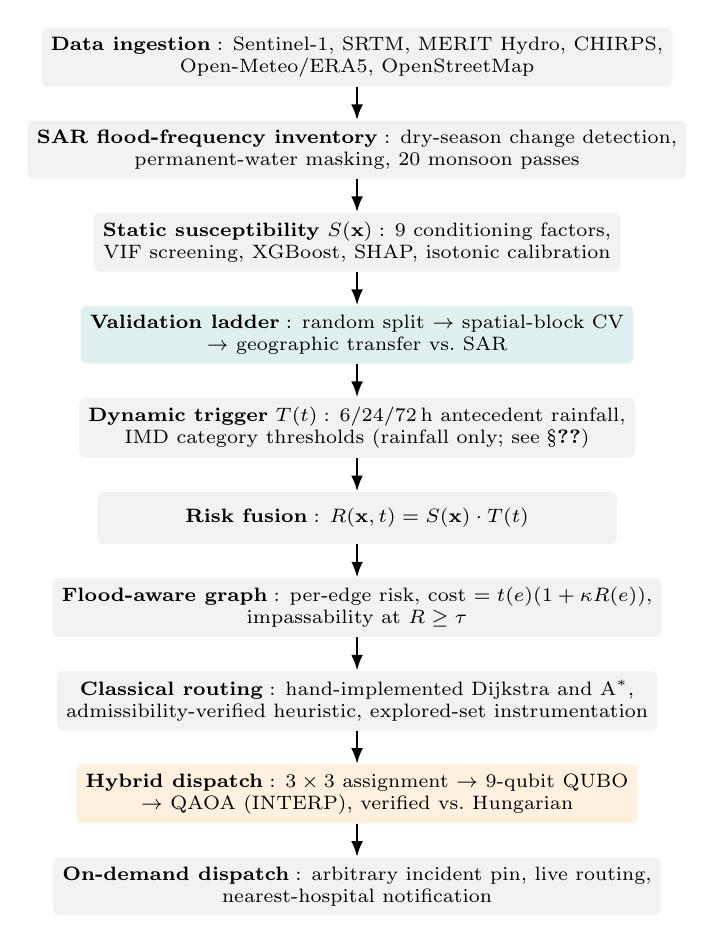
\begin{tikzpicture}[
  node distance=4.2mm and 8mm,
  % Borderless: a light fill alone separates the stages, so the diagram carries
  % no rule weight it does not need.
  box/.style={rounded corners=2pt, align=center, fill=black!5,
              font=\scriptsize, minimum width=6.6cm, minimum height=0.66cm},
  boxq/.style={box, fill=orange!12},
  boxv/.style={box, fill=teal!12},
  arr/.style={-{Latex[length=2mm]}, thick}
]
\node[box] (data) {\textbf{Data ingestion}\;: Sentinel-1, SRTM, MERIT Hydro, CHIRPS,\\ Open-Meteo/ERA5, OpenStreetMap};
\node[box, below=of data] (sar) {\textbf{SAR flood-frequency inventory}\;: dry-season change detection,\\ permanent-water masking, 20 monsoon passes};
\node[box, below=of sar] (model) {\textbf{Static susceptibility} $\Sx$\;: 9 conditioning factors,\\ VIF screening, XGBoost, SHAP, isotonic calibration};
\node[boxv, below=of model] (valid) {\textbf{Validation ladder}\;: random split $\rightarrow$ spatial-block CV\\ $\rightarrow$ geographic transfer vs.\ SAR};
\node[box, below=of valid] (trigger) {\textbf{Dynamic trigger} $\Tt$\;: 6/24/\SI{72}{\hour} antecedent rainfall,\\ IMD category thresholds (rainfall only; see \S\ref{sec:limitations})};
\node[box, below=of trigger] (fusion) {\textbf{Risk fusion}\;: $\Rxt=\Sx\cdot\Tt$};
\node[box, below=of fusion] (graph) {\textbf{Flood-aware graph}\;: per-edge risk, cost $=t(e)(1+\kappa R(e))$,\\ impassability at $R\ge\tau$};
\node[box, below=of graph] (route) {\textbf{Classical routing}\;: hand-implemented Dijkstra and A$^\ast$,\\ admissibility-verified heuristic, explored-set instrumentation};
\node[boxq, below=of route] (qaoa) {\textbf{Hybrid dispatch}\;: $3\times3$ assignment $\rightarrow$ 9-qubit QUBO\\ $\rightarrow$ QAOA (INTERP), verified vs.\ Hungarian};
\node[box, below=of qaoa] (pin) {\textbf{On-demand dispatch}\;: arbitrary incident pin, live routing,\\ nearest-hospital notification};

\foreach \a/\b in {data/sar, sar/model, model/valid, valid/trigger, trigger/fusion,
                   fusion/graph, graph/route, route/qaoa, qaoa/pin}
  \draw[arr] (\a) -- (\b);
\end{tikzpicture}
\caption{Pipeline. The two-stage split into a static SAR-trained surface and a
dynamic live trigger (shaded path through $\Sx$ and $\Tt$) is a direct
consequence of the twelve-day single-orbit revisit established in
Section~\ref{sec:intro}, not a modelling preference.}
\label{fig:architecture}
\end{figure}

\subsection{Why the risk model is decomposed}
\label{sec:method-decomp}
A fully spatiotemporal flood model would estimate inundation
$I(\mathbf{x},t)$ jointly in space and time. Fitting such a model requires
observations resolved at the timescale of the process. With one usable SAR orbit
at a twelve-day cadence, the observational record cannot constrain the temporal
dimension at all. We therefore factor the problem:
\begin{equation}
\Rxt \;=\; \Sx \cdot \Tt,
\qquad \Sx\in[0,1],\;\; \Tt\in[0,1],
\label{eq:fusion}
\end{equation}
where $\Sx$ is a time-invariant relative propensity estimated from the
\emph{frequency} of observed flooding across all available passes, and $\Tt$ is a
spatially uniform scalar estimated from meteorological data available at hourly
cadence. The factorisation assigns each term to the data that can actually
constrain it. Its cost is an explicit modelling assumption, that the spatial
pattern of relative risk does not change with event magnitude, which we return to
in Section~\ref{sec:limitations}.

\subsection{SAR flood-frequency inventory}
For each monsoon window (1 June--30 September 2024; 15 May--30 September 2025),
every Sentinel-1 GRD scene matching the fixed orbit geometry is speckle-filtered
with a \SI{30}{\metre} focal median and thresholded for open water:
\begin{equation}
W_k(\mathbf{x}) \;=\;
\mathbb{1}\!\left[\sigma^0_{VV,k}(\mathbf{x}) < \SI{-16}{\deci\bel}\right]\cdot
\mathbb{1}\!\left[\sigma^0_{VH,k}(\mathbf{x}) < \SI{-22}{\deci\bel}\right],
\label{eq:water}
\end{equation}
where $\sigma^0_{VV,k}$ and $\sigma^0_{VH,k}$ are calibrated backscatter
coefficients for pass $k$. A pixel counts as \emph{flooded} on pass $k$ only if it
is water then and dry in a January--February baseline, and is not permanent water:
\begin{equation}
F_k(\mathbf{x}) \;=\; W_k(\mathbf{x})\cdot\bigl(1-W_{\text{dry}}(\mathbf{x})\bigr)
\cdot\mathbb{1}\!\left[O_{\text{JRC}}(\mathbf{x}) < 80\%\right],
\label{eq:floodpass}
\end{equation}
with $O_{\text{JRC}}$ the JRC Global Surface Water occurrence~\citep{pekel2016}.
The inventory is the normalised frequency over the $K=20$ qualifying passes:
\begin{equation}
\Phi(\mathbf{x}) \;=\; \frac{1}{K}\sum_{k=1}^{K} F_k(\mathbf{x}) \;\in\; [0,1].
\label{eq:freq}
\end{equation}
Vectorising $\Phi>0$ over the routing window yields 201 polygons totalling
\SI{2.86}{\kilo\metre\squared} (Figure~\ref{fig:sar_inventory}). This area is a
\emph{lower bound} on flooding that occurred, not a flood map: it records only
what was inundated at the instants the satellite happened to look.

\begin{figure}[t]
\centering

\includegraphics[width=0.56\linewidth]{figures/sar_inventory.pdf}
\caption{The multi-temporal SAR flood inventory over the routing window: 201
polygons, \SI{2.86}{\kilo\metre\squared}, on a HAND backdrop with the channel
network and estuary. Observed flooding concentrates in the low-HAND corridors
flanking the Gurupura and Nethravathi and along the tidal margin.}
\label{fig:sar_inventory}
\end{figure}

\subsection{Conditioning factors and collinearity screening}
Twelve candidate factors were computed
(Figure~\ref{fig:conditioning}). TWI and the stream power index follow the
standard definitions~\citep{beven1979}:
\begin{equation}
\mathrm{TWI} = \ln\!\left(\frac{a}{\tan\beta}\right),
\qquad
\mathrm{SPI} = \ln\!\left(a\,\tan\beta\right),
\label{eq:twi}
\end{equation}
with $a$ the specific catchment area (\si{\metre\squared}) and $\beta$ the local
slope. HAND is the elevation of a pixel above the nearest hydrologically
connected drainage cell~\citep{renno2008,nobre2011}.

Collinearity was screened by variance inflation factor,
\begin{equation}
\mathrm{VIF}_j \;=\; \frac{1}{1-R_j^2},
\label{eq:vif}
\end{equation}
where $R_j^2$ is the coefficient of determination of factor $j$ regressed on all
others. As Table~\ref{tab:factors} shows, TWI and SPI are mutually collinear by
construction, both being functions of $a$ and $\tan\beta$; with both present they
score 16.22 and 14.50. Removing SPI reduces TWI to 1.49 and leaves every retained
factor below 3.5, comfortably under the conventional threshold of 10.

\begin{table*}[!t]
\centering\footnotesize
\caption{Conditioning factors. VIF is reported both with SPI present (11 numeric
candidates) and for the retained primary set. SPI is dropped because it and TWI
are algebraically coupled through specific catchment area and slope; removing one
resolves both.}
\label{tab:factors}
\small
\begin{tabular}{@{}llrrl@{}}
\toprule
\textbf{Factor} & \textbf{Definition / units} & \textbf{VIF (11)} & \textbf{VIF (9)} & \textbf{Source} \\
\midrule
Elevation & Height above sea level (\si{\metre}) & 3.87 & 3.46 & SRTM \\
Slope & Terrain gradient (\si{\degree}) & 3.72 & 1.54 & SRTM \\
Aspect & Slope azimuth (\si{\degree}) & 1.04 & 1.01 & SRTM \\
Curvature & Laplacian of elevation (--) & 1.10 & 1.10 & SRTM \\
HAND & Height above nearest drainage (\si{\metre}) & 2.91 & 2.85 & MERIT Hydro \\
TWI & $\ln(a/\tan\beta)$ (--) & 16.22 & 1.49 & MERIT Hydro \\
Distance to river & Euclidean distance to channel (\si{\metre}) & 2.71 & 2.71 & MERIT Hydro \\
Drainage density & Channel fraction in \SI{1}{\kilo\metre} neighbourhood (--) & 2.21 & 2.19 & MERIT Hydro \\
Annual rainfall & 2020--2024 mean (\si{\milli\metre}) & 2.16 & 2.14 & CHIRPS \\
\midrule
\multicolumn{5}{@{}l@{}}{\emph{Dropped:}} \\
SPI & $\ln(a\tan\beta)$ (--) & 14.50 & -- & VIF $>10$ \\
NDVI & Normalised difference vegetation index & 1.52 & -- & Confound (Sec.~\ref{sec:method-confound}) \\
Land cover & ESA WorldCover class & -- & -- & Confound (Sec.~\ref{sec:method-confound}) \\
\bottomrule
\end{tabular}
\end{table*}

\begin{figure*}[!t]
\centering

\includegraphics[width=\linewidth]{figures/conditioning_factors.pdf}
\caption{The nine conditioning factors of the primary model over the Mangaluru
window. The channel network is visible as low-slope, high-TWI, low-HAND
corridors; the coarse CHIRPS grid is apparent in the rainfall panel and is a
known resolution limit of that product.}
\label{fig:conditioning}
\end{figure*}

\subsection{Sampling with terrain-matched negatives}
Training points are drawn by stratified sampling, \num{1500} per class, under two
constraints. Positives require $\Phi(\mathbf{x})\ge 0.05$; negatives require
$\Phi(\mathbf{x})=0$ \emph{and} a distance of at least \SI{120}{\metre} from any
flood pixel, which removes the ambiguous halo around observed flooding. Both
classes are confined to a floodable-lowland domain,
\begin{equation}
\mathcal{D} \;=\; \bigl\{\mathbf{x} \;:\; z(\mathbf{x}) \le \SI{280}{\metre}
\;\wedge\; h(\mathbf{x}) \le \SI{80}{\metre}\bigr\},
\label{eq:domain}
\end{equation}
with $z$ elevation and $h$ HAND, both thresholds set at the 90th percentile of
the flood-pixel distribution. Without $\mathcal{D}$ the negative class would be
drawn largely from forested uplands, and the classifier could separate the
classes on elevation alone without learning anything flood-specific. This
elevation- and HAND-matching of negatives is, in our assessment, the single
decision that most affects whether the reported scores mean anything.

\subsection{A remote-sensing confound, and its removal}
\label{sec:method-confound}
The first model trained on all twelve factors reached a test ROC-AUC of 0.9878.
SHAP attribution, however, ranked land cover and NDVI as the two most important
predictors, ahead of elevation and HAND (Figure~\ref{fig:spatial}c). Inspecting
the sample explained why: within the floodable-lowland domain, non-flood pixels
are overwhelmingly closed-canopy vegetation. C-band SAR cannot observe standing
water beneath a closed canopy~\citep{townsend2002,tsyganskaya2018}. A pixel under
forest is therefore labelled ``not observed flooded'' for a sensing reason, not a
hydrological one, and a model given land cover can achieve high accuracy by
learning \emph{where SAR can see the ground}, not where water collects.

This is circularity, not signal, and it would have transferred a spurious model
into an operational routing system. We therefore define the primary feature set
as terrain and rainfall only, nine factors, and retain the twelve-factor model
solely as a sensitivity analysis. Section~\ref{sec:res-ablation} quantifies the
cost of this decision: 0.9878 to 0.9625 in test ROC-AUC, with the SHAP ranking
reverting to elevation, HAND, distance to river, rainfall and TWI, an ordering
consistent with the physical literature.

\subsection{Classifier, calibration and explanation}
Random forest~\citep{breiman2001} and XGBoost~\citep{chen2016} were trained on a
70/30 stratified split, with 5-fold cross-validation on the training portion.
XGBoost was selected on test ROC-AUC.

Raw tree-ensemble scores are ranking outputs, not probabilities
\citep{niculescu2005}, so we calibrate with isotonic
regression~\citep{zadrozny2002} fitted by cross-validation on the training split
alone, and evaluate with the Brier score~\citep{brier1950}. Because the training
sample is class-balanced while the landscape is not, the calibrated score is
tied to a $0.5$ prior; Section~\ref{sec:res-calibration} quantifies this and
applies the standard prior correction \citep{elkan2001,saerens2002}:
\begin{equation}
\mathrm{BS} \;=\; \frac{1}{n}\sum_{i=1}^{n}\bigl(\hat{p}_i - y_i\bigr)^2,
\label{eq:brier}
\end{equation}
with $\hat{p}_i$ the predicted probability and $y_i\in\{0,1\}$ the label. Isotonic
regression finds the monotone $g$ minimising $\sum_i (g(s_i)-y_i)^2$ over the
raw scores $s_i$, so calibration cannot reorder predictions and therefore cannot
alter AUC by construction.

Feature attribution uses SHAP values~\citep{lundberg2017}, the Shapley
decomposition of a prediction over feature subsets:
\begin{equation}
\phi_j \;=\; \sum_{\mathcal{S}\subseteq \mathcal{F}\setminus\{j\}}
\frac{|\mathcal{S}|!\,\bigl(|\mathcal{F}|-|\mathcal{S}|-1\bigr)!}{|\mathcal{F}|!}
\Bigl[f\bigl(\mathcal{S}\cup\{j\}\bigr) - f(\mathcal{S})\Bigr],
\label{eq:shap}
\end{equation}
with $\mathcal{F}$ the feature set; we report $\overline{|\phi_j|}$ over the test
split.

\subsection{The validation ladder}
\label{sec:method-validation}
Three successively stricter protocols are reported.

\textbf{(i) Random split.} Standard stratified 70/30 with 5-fold CV. Comparable
to published practice, and optimistic for the reasons below.

\textbf{(ii) Spatial-block cross-validation.} Samples are assigned to
$0.05^\circ$ ($\approx\SI{5.5}{\kilo\metre}$) blocks and whole blocks are held
out~\citep{roberts2017}, so no test point shares a neighbourhood with a training
point. The block size exceeds the terrain autocorrelation range in this setting.

\textbf{(iii) Geographic transfer.} The strictest test. The model is trained
\emph{only} on the \num{2640} labelled points outside the Mangaluru window,
predicts wall-to-wall inside it, and is scored against the SAR polygons observed
there. The model never sees a label from the evaluation area, which is what
deployment to a neighbouring taluk would demand.

For (iii) we report ROC-AUC, hit rate (probability of detection),
false-alarm ratio and critical success index:
\begin{equation}
\begin{aligned}
\mathrm{POD}&=\tfrac{\mathrm{TP}}{\mathrm{TP}+\mathrm{FN}}, \qquad
\mathrm{FAR}=\tfrac{\mathrm{FP}}{\mathrm{TP}+\mathrm{FP}}, \\[2pt]
\mathrm{CSI}&=\tfrac{\mathrm{TP}}{\mathrm{TP}+\mathrm{FP}+\mathrm{FN}},
\end{aligned}
\label{eq:contingency}
\end{equation}
together with the success-rate curve~\citep{chung2003}, the cumulative fraction
of observed flooding captured as the landscape is ranked by descending
susceptibility. Introduced for landslide-hazard validation and standard in
susceptibility mapping since, the success-rate curve is the appropriate headline
metric here, because FAR and CSI
are severely distorted by the fact that SAR-observed flooding covers only 1.1\%
of the window and absence of observation is not evidence of dryness.

\subsection{Dynamic trigger}
\label{sec:method-trigger}
The trigger maps antecedent rainfall to $[0,1]$ through three terms referenced to
India Meteorological Department daily-rainfall categories, without any parameter
fitted to the events it is later tested on:
\begin{equation}
\begin{aligned}
\Tt \;=\; \min\Bigl(\;
&\underbrace{0.5\,\tfrac{\min(P_{24},\,\theta_{\mathrm{VH}})}{\theta_{\mathrm{VH}}}}_{\text{daily intensity}}
\;+\; \underbrace{0.3\,\tfrac{\min(P_{72},\,\theta_{\mathrm{sat}})}{\theta_{\mathrm{sat}}}}_{\text{catchment saturation}} \\[2pt]
&+\; \underbrace{0.2\,\tfrac{\min(P_{6},\,\theta_{\mathrm{H}})}{\theta_{\mathrm{H}}}}_{\text{short burst}},
\;\; 1 \Bigr),
\end{aligned}
\label{eq:trigger}
\end{equation}
where $P_{6},P_{24},P_{72}$ are trailing rainfall totals (\si{\milli\metre}) over
6, 24 and \SI{72}{\hour}; $\theta_{\mathrm{H}}=\SI{64.5}{\milli\metre}$ (IMD
Heavy) and $\theta_{\mathrm{VH}}=\SI{115.6}{\milli\metre}$ (IMD Very Heavy) are
published category thresholds; and $\theta_{\mathrm{sat}}=\SI{200}{\milli\metre}$
is a saturation reference. We note explicitly that while $\theta_{\mathrm{H}}$
and $\theta_{\mathrm{VH}}$ are published IMD category boundaries, the three
weights and $\theta_{\mathrm{sat}}$ are chosen by us: $\theta_{\mathrm{sat}}$ is
a round value on the order of the wet-season soil-moisture storage of these
catchments, not a measured constant. Section~\ref{sec:res-trigger-sweep} sweeps
all four. The three-term structure encodes the physical premise
that a saturated catchment floods on less additional rain. Equation~\eqref{eq:trigger}
is monotone non-decreasing in each $P$ by construction, a property we verify
numerically rather than assert (Section~\ref{sec:res-trigger}). The outer
$\min(\cdot,1)$ is redundant at the operating weights, since they sum to one and
each term is individually capped, but is retained because
Section~\ref{sec:res-trigger-sweep} evaluates weightings for which it binds.

\subsection{Implementation}
The pipeline is Python 3.13 with pinned dependencies: \texttt{earthengine-api}
and \texttt{geemap} for server-side processing, \texttt{scikit-learn}
\citep{pedregosa2011}, \texttt{xgboost} \citep{chen2016} and \texttt{shap}
\citep{lundberg2017} for modelling, \texttt{osmnx} \citep{boeing2017} and
\texttt{networkx} for network acquisition and reference validation,
\texttt{geopandas}/\texttt{rasterio}/\texttt{shapely} for geometry,
\texttt{numpy} \citep{harris2020} and \texttt{scipy} \citep{virtanen2020} for the
statevector simulation and the Hungarian reference solver, and
\texttt{matplotlib} \citep{hunter2007} for all figures. Artifacts are built
by a dependency-aware Makefile, so a full rebuild regenerates every number and
figure reported here from source data. A suite of 80 automated tests encodes the
methodological invariants as executable assertions, including class balance and
domain confinement of the sample, $\mathrm{VIF}<10$ for all retained factors,
monotonicity of $\Tt$, heuristic admissibility, agreement of Dijkstra, A$^\ast$
and \texttt{networkx} on every benchmarked path, and equality of the QUBO ground
state with the Hungarian optimum. Every experiment reported here ran on one Apple
M3 Pro workstation with \SI{18}{\giga\byte} RAM. Apart from the server-side
raster work that Earth Engine performs on its own infrastructure, no additional
compute was needed.

%==============================================================================
\section{Results and Discussion}
\label{sec:results}

\subsection{Feature-set ablation: the price of removing circularity}
\label{sec:res-ablation}

Table~\ref{tab:ablation} reports the ablation ladder. The twelve-factor model is
the strongest by every metric, and is the model we discard. Its SHAP ranking
places land cover first and NDVI second; once both are removed the ranking
becomes elevation, HAND, distance to river, annual rainfall, TWI, which is the
ordering the flood-susceptibility literature reports on independent study
regions~\citep{arabameri2019,saha2021,aydin2022}. Dropping SPI on collinearity
grounds costs essentially nothing (0.9878 to 0.9872), confirming it carried no
independent information. Dropping NDVI and land cover costs 0.025 AUC and 0.038
$F_1$.

We regard the 0.9625 figure as the honest one and the 0.9878 as an artefact of
sensor physics. A reviewer comparing this work against papers reporting
0.98--0.99 on similar data should be aware that the difference may be a
methodological choice, not a modelling deficiency.

\paragraph{A smaller version of the same problem, in a factor we retained}
Having built the argument above, it would be inconsistent not to apply the same
scepticism to the surviving features, and one does not fully survive it. CHIRPS
has a $0.05^\circ$ ($\approx\SI{5.5}{\kilo\metre}$) grid, so the routing window
contains only 17 distinct rainfall values across \num{292125} pixels, yet SHAP
ranks \texttt{rain\_annual} fourth. A variable that coarse cannot be resolving
fine-scale hydrology. Measuring what it is actually doing: its correlation with
distance from the coast is $0.73$ and with elevation $0.33$, so within this
window it functions substantially as a smooth coast-to-inland gradient, that is,
a proxy for the orographic ramp, not a local rainfall signal.

It is not, however, empty. Leave-one-out retraining shows removing it costs
$0.0063$ AUC, the second largest of any single factor after elevation
($0.0173$), so it carries information the terrain variables do not. Our reading
is that at district scale the CHIRPS gradient encodes a real orographic
precipitation contrast that matters for susceptibility, while at city scale it
degenerates into a positional covariate. We retain it, because the model is
trained district-wide, and flag it here so the SHAP ranking is not
over-interpreted as evidence of fine-scale rainfall control. This is a weaker
version of the NDVI problem: a variable earning attribution partly for a reason
other than the one its name implies.

\begin{table*}[!t]
\centering\footnotesize
\caption{Feature-set ablation on the held-out test split ($n=900$). ``12F''
includes SPI, NDVI and land cover; ``11F'' drops SPI on VIF grounds; ``9F'' is
the primary terrain-and-rainfall model. All models are XGBoost with identical
hyperparameters and split.}
\label{tab:ablation}
\small
\begin{tabular}{@{}lrrrrrrl@{}}
\toprule
\textbf{Set} & \textbf{Acc.} & \textbf{Prec.} & \textbf{Rec.} & \textbf{$F_1$} &
\textbf{ROC-AUC} & \textbf{CV AUC} & \textbf{SHAP top-3} \\
\midrule
12F & 0.9456 & 0.9368 & 0.9556 & 0.9461 & 0.9878 & $0.9839\pm0.0092$ & lulc, ndvi, elevation \\
11F & 0.9478 & 0.9390 & 0.9578 & 0.9483 & 0.9872 & $0.9833\pm0.0098$ & lulc, ndvi, elevation \\
\textbf{9F} & 0.9111 & 0.9167 & 0.9044 & 0.9105 & 0.9625 & $0.9585\pm0.0154$ & elevation, hand, dist\_river \\
\bottomrule
\end{tabular}
\end{table*}

Model selection between random forest and XGBoost on the primary set is reported
in Table~\ref{tab:model} and Figure~\ref{fig:model_metrics}; the two are close,
and XGBoost is selected on test ROC-AUC. Its SHAP attribution
(Figure~\ref{fig:shap}) ranks elevation and HAND first, followed by channel
proximity, rainfall climatology and wetness, an ordering consistent with the
hydrological reading of the terms and free of the land-cover dominance that
characterised the discarded 12-factor model.

\begin{table*}[!t]
\centering\footnotesize
\caption{Primary (9-factor) model performance on the held-out test split
($n=900$).}
\label{tab:model}
\small
\begin{tabular}{@{}lrrrrrr@{}}
\toprule
\textbf{Model} & \textbf{Accuracy} & \textbf{Precision} & \textbf{Recall} &
\textbf{$F_1$} & \textbf{ROC-AUC} & \textbf{5-fold CV AUC} \\
\midrule
Random forest & 0.9033 & 0.9060 & 0.9000 & 0.9030 & 0.9618 & $0.9554\pm0.0110$ \\
\textbf{XGBoost} & \textbf{0.9111} & \textbf{0.9167} & \textbf{0.9044} &
\textbf{0.9105} & \textbf{0.9625} & $0.9534\pm0.0086$ \\
\bottomrule
\end{tabular}
\end{table*}

\begin{figure}[t]
\centering
\begin{subfigure}{0.48\textwidth}
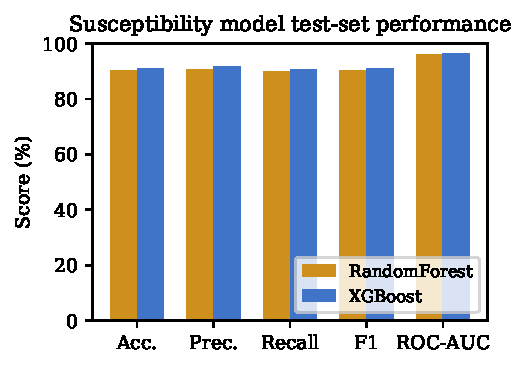
\includegraphics[width=\linewidth]{figures/model_metrics.pdf}
\caption{}\label{fig:model_metrics}
\end{subfigure}\hfill
\begin{subfigure}{0.48\textwidth}
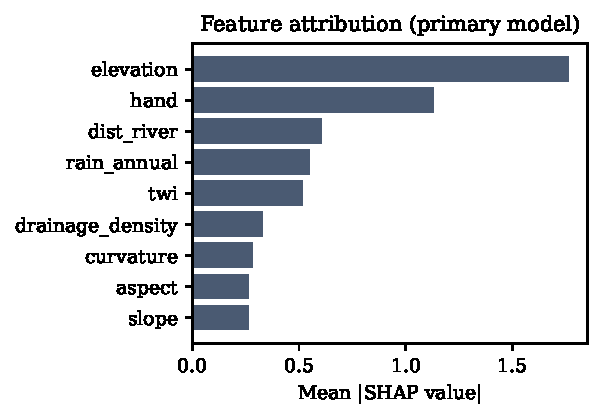
\includegraphics[width=\linewidth]{figures/shap_importance.pdf}
\caption{}\label{fig:shap}
\end{subfigure}
\caption{(a) Random forest versus XGBoost on the primary 9-factor set.
(b) SHAP attribution for the primary model: elevation and HAND dominate, followed
by channel proximity, rainfall climatology and wetness.}
\end{figure}

\subsection{Probability calibration, and what the score does \emph{not} mean}
\label{sec:res-calibration}
Isotonic calibration improved the Brier score from 0.0697 to 0.0683 and, being a
monotone transform, left ranking performance unchanged (ROC-AUC 0.9648). The
reliability diagram (Figure~\ref{fig:calibration}) tracks the diagonal across the
probability range.

It would be easy, and wrong, to conclude from this that $\Sx$ can be read as a
probability of flooding. The training sample is stratified \num{1500}/\num{1500},
so its implied base rate is exactly $0.5$ by construction, and isotonic
regression fitted on that split calibrates to a $0.5$ prior. The deployment
prevalence, measured as the SAR-observed flooded fraction of the routing window,
is $0.0111$ (Table~\ref{tab:transfer}). The calibrated score is therefore
well-behaved with respect to a reference population in which half the landscape
floods, which is not the landscape.

The consequence is measurable and, importantly, it partly explains a result we
initially attributed elsewhere. At a $0.5$ cut the balanced-prior model flags
34.3\% of the window as positive. Applying the standard prior
correction~\citep{elkan2001,saerens2002}, for a model trained at prior
$\pi_{\mathrm{tr}}$ and deployed at $\pi_{\mathrm{dep}}$,
\begin{equation}
p' \;=\; \frac{p\,\omega}{p\,\omega + (1-p)},
\qquad
\omega \;=\; \frac{\pi_{\mathrm{dep}}/(1-\pi_{\mathrm{dep}})}
                  {\pi_{\mathrm{tr}}/(1-\pi_{\mathrm{tr}})} \;=\; 0.0112,
\label{eq:priorshift}
\end{equation}
drops that to 3.66\% (Table~\ref{tab:prior}). Because \eqref{eq:priorshift} is
strictly increasing in $p$, ROC-AUC is invariant at 0.9648, which is the point:
the ranking was never in question, only the interpretation of its absolute level.

Section~\ref{sec:res-spatial} defends the high false-alarm ratio on the grounds
that absence of SAR observation is not evidence of dryness. That argument stands,
but it is not the whole explanation, and we correct it here: a substantial part
of the 34.3\% positive fraction is simply the balanced-prior artefact. We
therefore report $\Sx$ throughout as a \emph{relative exposure ranking}, which is
what the routing layer consumes and what the success-rate curve evaluates, and we
do not recommend thresholding it at 0.5 as though it were a posterior. An
operational deployment wanting absolute probabilities should apply
\eqref{eq:priorshift} with a locally estimated prevalence, bearing in mind that
the SAR-derived $\pi_{\mathrm{dep}}$ used here is itself a lower bound.

\begin{table*}[!t]
\centering\footnotesize
\caption{Effect of the training prior. The classifier is trained on a balanced
sample; the landscape is not balanced. The prior-corrected posterior changes what
a score means, not how scores rank.}
\label{tab:prior}
\small
\begin{tabular}{@{}lrr@{}}
\toprule
\textbf{Quantity} & \textbf{Balanced prior} & \textbf{Prevalence-corrected} \\
\midrule
Implied base rate & 0.500 & 0.0111 \\
Brier score (balanced test split) & 0.0683 & --- \\
ROC-AUC & 0.9648 & 0.9648 (invariant) \\
Landscape flagged at a 0.5 cut & 34.3\% & 3.66\% \\
Mean score over the window & 0.354 & 0.071 \\
99th percentile of the window & --- & 0.678 \\
\bottomrule
\end{tabular}
\end{table*}

\begin{figure}[t]
\centering
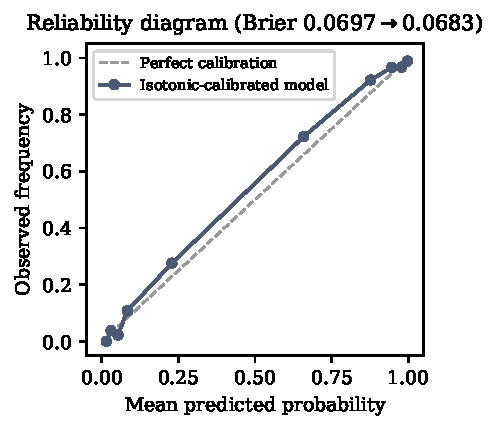
\includegraphics[width=0.48\linewidth]{figures/calibration.pdf}
\caption{Reliability diagram after isotonic calibration. Predicted probabilities
track observed frequencies across the range.}
\label{fig:calibration}
\end{figure}

\subsection{Spatial validation: how much skill is real}
\label{sec:res-spatial}

Table~\ref{tab:spatial} and Figure~\ref{fig:spatial} report the validation
ladder, and the pattern across it is the most methodologically interesting result
in this paper.

Under spatial-block cross-validation the primary model falls from 0.9585 to
0.9474, a drop of 1.16\%. This is small, and it means the model is not
substantially exploiting spatial autocorrelation: held-out geography costs it
about one point of AUC. Notably the twelve-factor model drops far \emph{less}
(0.30\%), which is not evidence that it generalises better. Land cover is so
strongly predictive of the SAR label that it swamps the spatial structure, so the
block-CV control has little left to remove. A spatial-CV score taken in isolation
would therefore have ranked the confounded model as the more robust one, which is
a caution worth recording: spatial validation controls for leakage through
geography, not for leakage through a sensor artefact.

Under the strictest test, geographic transfer, AUC falls to 0.871
(Table~\ref{tab:transfer}). Hit rate is high at 0.942, and the success-rate curve
(Figure~\ref{fig:sar_val}b) shows the top 10\% of the landscape by susceptibility
contains 49.5\% of all SAR-observed flooding and the top 20\% contains 77.6\%,
lifts of $4.9\times$ and $3.9\times$ over a random ranking. This is the number we
would defend operationally. Figure~\ref{fig:susceptibility} shows the two
surfaces side by side: the model trained entirely outside this window
reproduces the same drainage-following structure as the one trained on it,
which is the qualitative counterpart of that transfer score.

The false-alarm ratio of 0.970 requires care, not concealment. Observed
flood pixels are 1.1\% of the window, so at a 0.5 threshold the majority of
predicted-positive pixels are necessarily unobserved-flooded. More importantly,
under a twelve-day revisit a pixel outside the polygons means ``not seen
flooded'', never ``dry''. The FAR is therefore an upper bound on the true false
alarm rate and should not be read as a 97\% error rate; the AUC and the
success-rate curve, both of which use the full ranking rather than a threshold,
are the interpretable summaries.

\begin{table*}[!t]
\centering\footnotesize
\caption{Random versus spatial-block 5-fold cross-validation. Blocks are
$0.05^\circ$ squares; whole blocks are held out.}
\label{tab:spatial}
\small
\begin{tabular}{@{}lrrrr@{}}
\toprule
\textbf{Feature set} & \textbf{Random 5-fold AUC} & \textbf{Spatial-block AUC} &
\textbf{Drop} & \textbf{Drop (\%)} \\
\midrule
12F & $0.9839\pm0.0092$ & $0.9810\pm0.0052$ & 0.0030 & 0.30 \\
11F & $0.9833\pm0.0098$ & $0.9805\pm0.0059$ & 0.0028 & 0.29 \\
\textbf{9F} & $0.9585\pm0.0154$ & $0.9474\pm0.0039$ & 0.0111 & 1.16 \\
\bottomrule
\end{tabular}
\end{table*}

\begin{table*}[!t]
\centering
\caption{Geographic-transfer validation. The model is trained on the \num{2640}
labelled points \emph{outside} the Mangaluru window and scored against SAR
polygons inside it; \num{360} inside points are withheld entirely. Contingency
metrics use a 0.5 threshold.}
\label{tab:transfer}
\small
\begin{tabular}{@{}lr@{\qquad}lr@{}}
\toprule
\textbf{Quantity} & \textbf{Value} & \textbf{Quantity} & \textbf{Value} \\
\midrule
Training points (outside) & \num{2640} & ROC-AUC & 0.871 \\
Points withheld (inside) & \num{360} & Hit rate (POD) & 0.942 \\
Valid prediction pixels & \num{291546} & False-alarm ratio$^{\dagger}$ & 0.970 \\
Observed-flood pixels & \num{3227} (1.11\%) & Critical success index$^{\dagger}$ & 0.030 \\
TP / FN & \num{3040} / \num{187} & Flooding in top 10\% area & 49.5\% \\
TN / FP & \num{191393} / \num{96926} & Flooding in top 20\% area & 77.6\% \\
\bottomrule
\multicolumn{4}{@{}p{13.5cm}@{}}{\footnotesize $^{\dagger}$Upper and lower bounds
respectively: SAR observes flooding only on its twelve-day revisit, so a pixel
outside the polygons is ``not observed flooded'', not ``dry''.}
\end{tabular}
\end{table*}

\begin{figure}[t]
\centering

\includegraphics[width=\linewidth]{figures/spatial_validation.pdf}
\caption{(a) Feature-set ablation. (b) Random versus spatial-block
cross-validation; the confounded 12F model drops least, because land cover
dominates the spatial signal. (c) SHAP top-6 for the 9-factor and 12-factor
models side by side, showing land cover and NDVI displacing terrain in the
confounded model.}
\label{fig:spatial}
\end{figure}

\begin{figure}[t]
\centering

\includegraphics[width=\linewidth]{figures/sar_validation.pdf}
\caption{Geographic transfer. (a) ROC against SAR-observed flooding for a model
trained entirely outside the evaluation window. (b) Success-rate curve: the
highest-susceptibility 10\% of the landscape contains 49.5\% of observed
flooding.}
\label{fig:sar_val}
\end{figure}

\begin{figure*}[!t]
\centering

\includegraphics[width=\linewidth]{figures/susceptibility_surface.pdf}
\caption{(a) The calibrated susceptibility surface $\Sx$ over the Mangaluru
window with SAR-observed flooding outlined. (b) The geographic-transfer
prediction from a model trained outside this window. The two surfaces are
visually similar, which is the qualitative counterpart of the transfer AUC of
0.871.}
\label{fig:susceptibility}
\end{figure*}

\subsection{Trigger validation and its discriminative limit}
\label{sec:res-trigger}

Table~\ref{tab:trigger} publishes the complete input record behind every trigger
value, which we consider necessary: a trigger whose inputs are not shown cannot
be checked. Equation~\eqref{eq:trigger} is verified monotone under uniform
rainfall scaling ($T = 0.000, 0.063, 0.125, 0.251, 0.502, 0.924, 1.000$ for
scale factors $0$ to $8$).

The ordering test passes. Both documented floods score above an ordinary wet day
($T=0.133$) and a dry baseline ($T=0.000$), with no parameter fitted to them.
Notably the two events arrive at high $T$ by different routes: May 2025 through
daily intensity (\SI{87.2}{\milli\metre}/\SI{24}{\hour}, IMD Heavy) and
August 2024 through saturation (\SI{216.9}{\milli\metre}/\SI{72}{\hour}) despite
a merely Moderate 24-hour total. A single-threshold rainfall alarm keyed to
24-hour totals would have ranked August 2024 below an ordinary heavy day; the
three-term structure is what recovers it.

The adversarial case is where the result is weaker, and we report it as measured.
A deliberately chosen heavy-rain day with no reported flooding
(15 July 2025; \SI{66.8}{\milli\metre}/\SI{24}{\hour}, IMD Heavy) scores
$T=0.551$, only $0.011$ below the August 2024 flood. The trigger separates flood
from non-flood conditions strongly but separates flood from
\emph{heavy-rain-without-flood} barely at all. Figure~\ref{fig:trigger}b shows
why, and also suggests the remedy: the discriminating variable is the 72-hour
saturation total (\num{216.9} and \SI{205.6}{\milli\metre} for the two floods
versus \SI{116.8}{\milli\metre} for the non-flood day), while the burst term
actively works against separation, being highest of all on the non-flood day
(\SI{28.0}{\milli\metre}/\SI{6}{\hour}). Re-weighting toward saturation would
widen the margin, but doing so using these events would convert a validated
trigger into a fitted one, so we report the limitation rather than tune it away.

\begin{table*}[!t]
\centering\footnotesize
\caption{Complete trigger inputs, from the ERA5 archive via Open-Meteo at
Mangaluru ($12.87^\circ$N, $74.84^\circ$E). Weighted terms are the three
components of Equation~\eqref{eq:trigger}. No parameter is fitted to these
events.}
\label{tab:trigger}
\small
\setlength{\tabcolsep}{4pt}
\begin{tabular}{@{}llrrrlrrrr@{}}
\toprule
\multirow{2}{*}{\textbf{Scenario}} & \multirow{2}{*}{\textbf{Class}} &
\multicolumn{3}{c}{\textbf{Rainfall (\si{\milli\metre})}} &
\multirow{2}{*}{\textbf{IMD (24\,h)}} &
\multicolumn{3}{c}{\textbf{Weighted terms}} & \multirow{2}{*}{$\boldsymbol{T}$} \\
\cmidrule(lr){3-5}\cmidrule(lr){7-9}
 & & \textbf{6\,h} & \textbf{24\,h} & \textbf{72\,h} & &
 \textbf{daily} & \textbf{sat.} & \textbf{burst} & \\
\midrule
May 2025 Mangaluru urban & flood & 7.6 & 87.2 & 205.6 & Heavy & 0.377 & 0.300 & 0.024 & \textbf{0.701} \\
Aug 2024 Nethravathi river & flood & 10.1 & 53.4 & 216.9 & Moderate & 0.231 & 0.300 & 0.031 & \textbf{0.562} \\
15 Jul 2025 heavy rain & no flood & 28.0 & 66.8 & 116.8 & Heavy & 0.289 & 0.175 & 0.087 & 0.551 \\
6 Sep 2025 ordinary wet & wet & 3.2 & 11.0 & 50.0 & Light & 0.048 & 0.075 & 0.010 & 0.133 \\
16 Feb 2025 dry baseline & dry & 0.0 & 0.0 & 0.0 & No rain & 0.000 & 0.000 & 0.000 & 0.000 \\
\bottomrule
\end{tabular}
\end{table*}

\begin{figure*}[!t]
\centering

\includegraphics[width=\linewidth]{figures/trigger_anatomy.pdf}
\caption{(a) Decomposition of $\Tt$ into its three weighted terms. (b) The
measured rainfall inputs. The two documented floods exceed
\SI{200}{\milli\metre} of 72-hour antecedent rainfall; the heavy-rain non-flood
day reaches only \SI{116.8}{\milli\metre} despite the largest 6-hour burst in the
set, identifying catchment saturation as the discriminating variable.
(c) Mean adversarial margin across the weight simplex as a function of the
saturation weight, at $\theta_{\mathrm{sat}}=\SI{200}{\milli\metre}$. The
operating point sits almost exactly at the zero crossing.}
\label{fig:trigger}
\end{figure*}

\subsubsection*{Sensitivity of the trigger's own constants}
\label{sec:res-trigger-sweep}
Equation~\eqref{eq:trigger} contains four author-chosen constants: the three
weights and $\theta_{\mathrm{sat}}$. Only $\theta_{\mathrm{H}}$ and
$\theta_{\mathrm{VH}}$ are externally published. Having swept the routing
constants, it would be inconsistent not to sweep these, particularly since they
govern the paper's weakest result. Table~\ref{tab:triggersweep} reports 231
weight triples on the simplex at 0.05 resolution crossed with five values of
$\theta_{\mathrm{sat}}$, evaluated on the same five scenarios.

Two findings. First, the \emph{easy} discrimination is completely robust: floods
rank above the ordinary wet day and the dry baseline in all \num{1155} settings,
so that result is a property of the input data, not of the weights.
Second, the \emph{hard} discrimination is governed almost entirely by one weight.
The adversarial margin rises monotonically from $-0.200$ at zero saturation
weight to $+0.416$ at unit saturation weight
(Figure~\ref{fig:trigger}c), and is positive in only 374 of \num{1155} settings.
The operating point, at saturation weight 0.3, sits essentially on the zero
crossing, which is why its margin is a marginal $+0.011$.

This converts the qualitative diagnosis of the previous subsection into a
measurement: the 72-hour antecedent term carries the flood-versus-heavy-rain
signal, and the operating weights under-use it. We deliberately do \emph{not}
adopt the optimum. Choosing weights to maximise separation on the same five
events the trigger is validated against would convert a validated component into
a fitted one and forfeit the property this paper claims for it. Re-weighting
requires an independent event set, which we identify as future work.

\begin{table*}[!t]
\centering\footnotesize
\caption{Sensitivity of the trigger to its four unpublished constants, over 231
weight triples $\times$ 5 values of $\theta_{\mathrm{sat}}$. ``Adversarial
margin'' is $\min_{\text{floods}} T$ minus $T$ for the heavy-rain non-flood day;
``ordinary margin'' is against the ordinary wet day. The optimum is reported for
information and is not adopted.}
\label{tab:triggersweep}
\small
\begin{tabular}{@{}llrr@{}}
\toprule
\textbf{Setting} & \textbf{Weights (daily/sat./burst), $\theta_{\mathrm{sat}}$} &
\textbf{Adversarial} & \textbf{Ordinary} \\
\midrule
\textbf{Operating point (adopted)} & 0.50 / 0.30 / 0.20, \SI{200}{\milli\metre} & $+0.011$ & $+0.430$ \\
Best over the sweep (not adopted) & 0.00 / 1.00 / 0.00, \SI{200}{\milli\metre} & $+0.416$ & $+0.610$ \\
Worst over the sweep & 0.00 / 0.00 / 1.00, \SI{100}{\milli\metre} & $-0.316$ & $+0.062$ \\
\midrule
\multicolumn{2}{@{}l}{Settings with correct flood $>$ ordinary $>$ dry ordering} & \multicolumn{2}{r}{\num{1155} / \num{1155}} \\
\multicolumn{2}{@{}l}{Settings with a positive adversarial margin} & \multicolumn{2}{r}{374 / \num{1155}} \\
\multicolumn{2}{@{}l}{Settings with an adversarial margin above 0.05} & \multicolumn{2}{r}{277 / \num{1155}} \\
\bottomrule
\end{tabular}
\end{table*}

\subsection{Comparison with prior work}
Reported flood-susceptibility AUCs in the literature cluster between 0.85 and
0.95~\cite{tehrany2014,khosravi2018,arabameri2019,saha2021,aydin2022}. Our
confounded 12-factor model would sit above that range at 0.9878, and our
primary model sits inside it at 0.9625. We regard the second number as the
comparable one, and note that most reported figures are random-split values
whose spatial-block and transfer equivalents are unknown, which is precisely the
comparison Section~\ref{sec:res-spatial} argues the field should be making.

\subsection{Limitations}
\label{sec:limitations}
\begin{itemize}
\item \textbf{Susceptibility is not depth.} $\Sx$ and $\Rxt$ are relative
      exposure indices in $[0,1]$, not water depth. A calibrated depth
      regression, in the direction of Sadhwani and Eldho~\cite{sadhwani2026},
      is the clearest strengthening step.
\item \textbf{The calibrated score is prior-dependent.} It is calibrated to the
      balanced training prior, not to landscape prevalence, and must be
      prior-corrected before being read as a probability.
\item \textbf{The trigger is a single regional scalar} and uses rainfall only;
      tide is acquired by the live system but does not enter $\Tt$. Scenarios
      therefore differ in intensity, not in spatial pattern.
\item \textbf{The trigger's free constants are its weakest point.} Three weights
      and a saturation reference are author-chosen, and the flood versus
      heavy-rain margin is governed almost entirely by the saturation term.
\item \textbf{Geographic transfer here is within-district}, across a city
      boundary rather than across a climatic or geomorphic regime.
\item \textbf{SAR absence is not evidence of dryness.} The inventory is a lower
      bound set by a twelve-day revisit.
\end{itemize}
\section{Conclusions}
This paper built the static half of a two-stage flood-risk model for a district
where the satellite record forbids per-event mapping, and then spent most of its
effort trying to falsify it.

\begin{enumerate}
\item \textbf{A 12-factor model reaching ROC-AUC 0.9878 was discarded.} SHAP
      attribution ranked land cover and NDVI first, and the non-flooded lowland
      of this district is predominantly closed canopy, so the model was learning
      where SAR can see the ground. Removing the confound costs 0.025 AUC and is
      mandatory.
\item \textbf{Stricter validation lowered the number three times.} 0.9625 on a
      random split, 0.9474 under spatial-block cross-validation, 0.871 on
      geographic transfer. The last of these is the one an operational
      deployment would experience, and its highest-susceptibility tenth still
      contains 49.5\% of observed flooding.
\item \textbf{The calibrated score is not a flood probability.} Isotonic
      calibration on a balanced sample targets a 50\% prior against a landscape
      prevalence of 1.11\%; the correction changes what the number means without
      changing the ranking.
\item \textbf{The trigger orders real events without being fitted to them},
      but separates a documented flood from a heavy-rain non-flood day by only
      0.011, and the diagnostic identifies the 72-hour saturation term as the
      variable carrying the signal.
\end{enumerate}

The broader claim is methodological: each protocol we applied removed a specific,
nameable way the previous figure was optimistic, and the sequence is more useful
to a practitioner than its first term. Part~II~\cite{partii} takes the resulting
risk surface into the emergency-response layer, where the same discipline is
applied to routing and dispatch.

\balance
\begin{thebibliography}{99}
\setlength{\itemsep}{1pt}

\bibitem[Chandrashekar and Shetty(2018)]{chandrashekar2018}
V.~D.~Chandrashekar, A.~Shetty.
Trends in extreme rainfall over ecologically sensitive Western Ghats and coastal
regions of Karnataka: an observational assessment.
\emph{Arabian Journal of Geosciences}, 11:327, 2018.
\href{https://doi.org/10.1007/s12517-018-3700-6}{doi:10.1007/s12517-018-3700-6}.

\bibitem[Chandana and Chandan(2023)]{chandana2023}
S.~Chandana, M.~C.~Chandan.
Hydrological implications of LULC changes in the Netravathi river basin:
insights from SWAT modeling.
In \emph{2023 IEEE India Geoscience and Remote Sensing Symposium (InGARSS)},
pages 1--4, 2023.
\href{https://doi.org/10.1109/InGARSS59135.2023.10490324}{doi:10.1109/InGARSS59135.2023.10490324}.

\bibitem[Babar and Ramesh(2015)]{babar2015}
S.~Babar, H.~Ramesh.
Streamflow response to land use--land cover change over the Nethravathi River
basin, India.
\emph{Journal of Hydrologic Engineering}, 20(10):05015002, 2015.
\href{https://doi.org/10.1061/(ASCE)HE.1943-5584.0001177}{doi:10.1061/(ASCE)HE.1943-5584.0001177}.

\bibitem[Naik et al.(2022)]{naik2022}
N.~Naik, K.~Chandrasekaran, V.~M.~Sundaram, P.~Panneer.
Dual attention guided deep encoder-decoder network for change analysis in land
use/land cover for Dakshina Kannada District, Karnataka, India.
\emph{Environmental Earth Sciences}, 82(1):33, 2022.
\href{https://doi.org/10.1007/s12665-022-10713-1}{doi:10.1007/s12665-022-10713-1}.

\bibitem[Nirmala(2026)]{nirmala2026}
R.~Nirmala.
Flood susceptibility assessment of Nethravathi River basin, Karnataka, through
GIS-AHP technique.
In \emph{Sustainability Solutions}, pages 643--661. Springer, 2026.
\href{https://doi.org/10.1007/978-3-032-11300-9_27}{doi:10.1007/978-3-032-11300-9\_27}.

\bibitem[Tehrany et al.(2014)]{tehrany2014}
M.~S.~Tehrany, B.~Pradhan, M.~N.~Jebur.
Flood susceptibility mapping using a novel ensemble weights-of-evidence and
support vector machine models in GIS.
\emph{Journal of Hydrology}, 512:332--343, 2014.

\bibitem[Khosravi et al.(2018)]{khosravi2018}
K.~Khosravi, B.~T.~Pham, K.~Chapi, A.~Shirzadi, H.~Shahabi, I.~Revhaug,
I.~Prakash, D.~T.~Bui.
A comparative assessment of decision trees algorithms for flash flood
susceptibility modeling at Haraz watershed, northern Iran.
\emph{Science of the Total Environment}, 627:744--755, 2018.

\bibitem[Arabameri et al.(2019)]{arabameri2019}
A.~Arabameri, K.~Rezaei, A.~Cerd\`a, C.~Conoscenti, Z.~Kalantari.
A comparison of statistical methods and multi-criteria decision making to map
flood hazard susceptibility in Northern Iran.
\emph{Science of the Total Environment}, 660:443--458, 2019.

\bibitem[Saha et al.(2021)]{saha2021}
A.~Saha, S.~Pal, A.~Arabameri, T.~Blaschke, S.~Panahi, I.~Chowdhuri,
R.~Chakrabortty, R.~Costache, A.~Arora.
Flood susceptibility assessment using novel ensemble of hyperpipes and support
vector regression algorithms.
\emph{Water}, 13(2):241, 2021.
\href{https://doi.org/10.3390/w13020241}{doi:10.3390/w13020241}.

\bibitem[Lundberg and Lee(2017)]{lundberg2017}
S.~M.~Lundberg, S.-I.~Lee.
A unified approach to interpreting model predictions.
In \emph{Advances in Neural Information Processing Systems 30}, 2017.

\bibitem[Aydin and Iban(2023)]{aydin2022}
H.~E.~Aydin, M.~C.~Iban.
Predicting and analyzing flood susceptibility using boosting-based ensemble
machine learning algorithms with SHapley Additive exPlanations.
\emph{Natural Hazards}, 116:2957--2991, 2023.
\href{https://doi.org/10.1007/s11069-022-05793-y}{doi:10.1007/s11069-022-05793-y}.

\bibitem[Seydi et al.(2023)]{seydi2023}
S.~T.~Seydi, Y.~Kanani-Sadat, M.~Hasanlou, R.~Sahraei, J.~Chanussot,
M.~Amani.
Comparison of machine learning algorithms for flood susceptibility mapping.
\emph{Remote Sensing}, 15(1):192, 2023.

\bibitem[Torres et al.(2012)]{torres2012}
R.~Torres, P.~Snoeij, D.~Geudtner, et al.
GMES Sentinel-1 mission.
\emph{Remote Sensing of Environment}, 120:9--24, 2012.
\href{https://doi.org/10.1016/j.rse.2011.05.028}{doi:10.1016/j.rse.2011.05.028}.

\bibitem[Arora et al.(2023)]{arora2023}
M.~Arora, S.~Sahoo, C.~M.~Bhatt, P.~K.~Litoria, B.~Pateriya.
Rapid flood inundation mapping and impact assessment using Sentinel-1 SAR data
over Ghaggar River basin of Punjab, India.
\emph{Journal of Earth System Science}, 132(4):183, 2023.
\href{https://doi.org/10.1007/s12040-023-02199-7}{doi:10.1007/s12040-023-02199-7}.

\bibitem[Roberts et al.(2017)]{roberts2017}
D.~R.~Roberts et al.
Cross-validation strategies for data with temporal, spatial, hierarchical, or
phylogenetic structure.
\emph{Ecography}, 40(8):913--929, 2017.

\bibitem[Ploton et al.(2020)]{ploton2020}
P.~Ploton et al.
Spatial validation reveals poor predictive performance of large-scale ecological
mapping models.
\emph{Nature Communications}, 11:4540, 2020.

\bibitem[Meyer and Pebesma(2021)]{meyer2021}
H.~Meyer, E.~Pebesma.
Predicting into unknown space? Estimating the area of applicability of spatial
prediction models.
\emph{Methods in Ecology and Evolution}, 12(9):1620--1633, 2021.

\bibitem[Companion(2026b)]{partii} Authors. Spatiotemporal flood risk modelling under a single-orbit SAR constraint, Part~II: Flood-aware emergency routing and hybrid quantum dispatch. \emph{Companion paper, submitted}.

\bibitem[Wang et al.(2020)]{wang2020}
Y.~Wang, Z.~Fang, H.~Hong, L.~Peng.
Flood susceptibility mapping using convolutional neural network frameworks.
\emph{Journal of Hydrology}, 582:124482, 2020.

\bibitem[Avand et al.(2021)]{avand2021}
M.~Avand, H.~Moradi, M.~Ramazanzadeh~Lasboyee.
Using machine learning models, remote sensing, and GIS to investigate the effects
of changing climates and land uses on flood probability.
\emph{Journal of Hydrology}, 595:125663, 2021.

\bibitem[Beven and Kirkby(1979)]{beven1979}
K.~J.~Beven, M.~J.~Kirkby.
A physically based, variable contributing area model of basin hydrology.
\emph{Hydrological Sciences Bulletin}, 24(1):43--69, 1979.

\bibitem[Renn\'o et al.(2008)]{renno2008}
C.~D.~Renn\'o, A.~D.~Nobre, L.~A.~Cuartas, J.~V.~Soares, M.~G.~Hodnett,
J.~Tomasella, M.~J.~Waterloo.
HAND, a new terrain descriptor using SRTM-DEM: mapping terra-firme rainforest
environments in Amazonia.
\emph{Remote Sensing of Environment}, 112(9):3469--3481, 2008.

\bibitem[Nobre et al.(2011)]{nobre2011}
A.~D.~Nobre, L.~A.~Cuartas, M.~Hodnett, C.~D.~Renn\'o, G.~Rodrigues, A.~Silveira,
M.~Waterloo, S.~Saleska.
Height Above the Nearest Drainage: a hydrologically relevant new terrain model.
\emph{Journal of Hydrology}, 404(1--2):13--29, 2011.

\bibitem[Martinis et al.(2009)]{martinis2009}
S.~Martinis, A.~Twele, S.~Voigt.
Towards operational near real-time flood detection using a split-based automatic
thresholding procedure on high resolution TerraSAR-X data.
\emph{Natural Hazards and Earth System Sciences}, 9:303--314, 2009.

\bibitem[Twele et al.(2016)]{twele2016}
A.~Twele, W.~Cao, S.~Plank, S.~Martinis.
Sentinel-1-based flood mapping: a fully automated processing chain.
\emph{International Journal of Remote Sensing}, 37(13):2990--3004, 2016.

\bibitem[Shen et al.(2019)]{shen2019}
X.~Shen, D.~Wang, K.~Mao, E.~Anagnostou, Y.~Hong.
Inundation extent mapping by synthetic aperture radar: a review.
\emph{Remote Sensing}, 11(7):879, 2019.

\bibitem[Pekel et al.(2016)]{pekel2016}
J.-F.~Pekel, A.~Cottam, N.~Gorelick, A.~S.~Belward.
High-resolution mapping of global surface water and its long-term changes.
\emph{Nature}, 540:418--422, 2016.

\bibitem[Townsend(2002)]{townsend2002}
P.~A.~Townsend.
Relationships between forest structure and the detection of flood inundation in
forested wetlands using C-band SAR.
\emph{International Journal of Remote Sensing}, 23(3):443--460, 2002.

\bibitem[Tsyganskaya et al.(2018)]{tsyganskaya2018}
V.~Tsyganskaya, S.~Martinis, P.~Marzahn, R.~Ludwig.
SAR-based detection of flooded vegetation: a review of characteristics and
approaches.
\emph{International Journal of Remote Sensing}, 39(8):2255--2293, 2018.

\bibitem[Donchyts et al.(2016)]{donchyts2016}
G.~Donchyts, F.~Baart, H.~Winsemius, N.~Gorelick, J.~Kwadijk, N.~van~de~Giesen.
Earth's surface water change over the past 30 years.
\emph{Nature Climate Change}, 6:810--813, 2016.

\bibitem[Sadhwani and Eldho(2026)]{sadhwani2026}
K.~Sadhwani, T.~I.~Eldho.
Machine learning-driven flood hazard assessment: integrating SAR and elevation
data for inundation mapping and depth estimation.
\emph{Natural Hazards}, 122:177, 2026.
\href{https://doi.org/10.1007/s11069-025-07949-y}{doi:10.1007/s11069-025-07949-y}.

\bibitem[Gorelick et al.(2017)]{gorelick2017}
N.~Gorelick, M.~Hancher, M.~Dixon, S.~Ilyushchenko, D.~Thau, R.~Moore.
Google Earth Engine: planetary-scale geospatial analysis for everyone.
\emph{Remote Sensing of Environment}, 202:18--27, 2017.

\bibitem[Farr et al.(2007)]{farr2007}
T.~G.~Farr et al.
The Shuttle Radar Topography Mission.
\emph{Reviews of Geophysics}, 45(2):RG2004, 2007.

\bibitem[Yamazaki et al.(2019)]{yamazaki2019}
D.~Yamazaki, D.~Ikeshima, J.~Sosa, P.~D.~Bates, G.~H.~Allen, T.~M.~Pavelsky.
MERIT Hydro: a high-resolution global hydrography map based on latest topography
datasets.
\emph{Water Resources Research}, 55(6):5053--5073, 2019.

\bibitem[Funk et al.(2015)]{funk2015}
C.~Funk et al.
The climate hazards infrared precipitation with stations: a new environmental
record for monitoring extremes.
\emph{Scientific Data}, 2:150066, 2015.

\bibitem[Zanaga et al.(2021)]{zanaga2021}
D.~Zanaga et al. ESA WorldCover 10\,m 2020 v100. Zenodo, 2021.
\href{https://doi.org/10.5281/zenodo.5571936}{doi:10.5281/zenodo.5571936}.

\bibitem[Hersbach et al.(2020)]{hersbach2020}
H.~Hersbach, B.~Bell, P.~Berrisford, et al.
The ERA5 global reanalysis.
\emph{Quarterly Journal of the Royal Meteorological Society}, 146(730):1999--2049, 2020.
\href{https://doi.org/10.1002/qj.3803}{doi:10.1002/qj.3803}.

\bibitem[Boeing(2017)]{boeing2017}
G.~Boeing.
OSMnx: New methods for acquiring, constructing, analyzing, and visualizing
complex street networks.
\emph{Computers, Environment and Urban Systems}, 65:126--139, 2017.
\href{https://doi.org/10.1016/j.compenvurbsys.2017.05.004}{doi:10.1016/j.compenvurbsys.2017.05.004}.

\bibitem[Breiman(2001)]{breiman2001}
L.~Breiman. Random forests. \emph{Machine Learning}, 45(1):5--32, 2001.

\bibitem[Chen and Guestrin(2016)]{chen2016}
T.~Chen, C.~Guestrin.
XGBoost: A scalable tree boosting system.
In \emph{Proc.\ 22nd ACM SIGKDD}, pages 785--794, 2016.

\bibitem[Niculescu-Mizil and Caruana(2005)]{niculescu2005}
A.~Niculescu-Mizil, R.~Caruana.
Predicting good probabilities with supervised learning.
In \emph{Proc.\ 22nd International Conference on Machine Learning (ICML)},
pages 625--632, 2005.
\href{https://doi.org/10.1145/1102351.1102430}{doi:10.1145/1102351.1102430}.

\bibitem[Zadrozny and Elkan(2002)]{zadrozny2002}
B.~Zadrozny, C.~Elkan.
Transforming classifier scores into accurate multiclass probability estimates.
In \emph{Proc.\ 8th ACM SIGKDD}, pages 694--699, 2002.

\bibitem[Brier(1950)]{brier1950}
G.~W.~Brier.
Verification of forecasts expressed in terms of probability.
\emph{Monthly Weather Review}, 78(1):1--3, 1950.

\bibitem[Elkan(2001)]{elkan2001}
C.~Elkan.
The foundations of cost-sensitive learning.
In \emph{Proc.\ 17th International Joint Conference on Artificial Intelligence
(IJCAI)}, pages 973--978, 2001.

\bibitem[Saerens et al.(2002)]{saerens2002}
M.~Saerens, P.~Latinne, C.~Decaestecker.
Adjusting the outputs of a classifier to new a priori probabilities: a simple
procedure.
\emph{Neural Computation}, 14(1):21--41, 2002.
\href{https://doi.org/10.1162/089976602753284446}{doi:10.1162/089976602753284446}.

\bibitem[Chung and Fabbri(2003)]{chung2003}
C.-J.~F.~Chung, A.~G.~Fabbri.
Validation of spatial prediction models for landslide hazard mapping.
\emph{Natural Hazards}, 30(3):451--472, 2003.
\href{https://doi.org/10.1023/B:NHAZ.0000007172.62651.2b}{doi:10.1023/B:NHAZ.0000007172.62651.2b}.

\bibitem[Pedregosa et al.(2011)]{pedregosa2011}
F.~Pedregosa, G.~Varoquaux, A.~Gramfort, et al.
Scikit-learn: Machine learning in Python.
\emph{Journal of Machine Learning Research}, 12:2825--2830, 2011.

\bibitem[Harris et al.(2020)]{harris2020}
C.~R.~Harris, K.~J.~Millman, S.~J.~van~der~Walt, et al.
Array programming with NumPy.
\emph{Nature}, 585:357--362, 2020.
\href{https://doi.org/10.1038/s41586-020-2649-2}{doi:10.1038/s41586-020-2649-2}.

\bibitem[Virtanen et al.(2020)]{virtanen2020}
P.~Virtanen, R.~Gommers, T.~E.~Oliphant, et al.
SciPy 1.0: Fundamental algorithms for scientific computing in Python.
\emph{Nature Methods}, 17:261--272, 2020.
\href{https://doi.org/10.1038/s41592-019-0686-2}{doi:10.1038/s41592-019-0686-2}.

\bibitem[Hunter(2007)]{hunter2007}
J.~D.~Hunter.
Matplotlib: A 2D graphics environment.
\emph{Computing in Science \& Engineering}, 9(3):90--95, 2007.
\href{https://doi.org/10.1109/MCSE.2007.55}{doi:10.1109/MCSE.2007.55}.

\end{thebibliography}

\end{document}
